\documentclass[11pt]{article}
\usepackage[margin=0.68in]{geometry}
\usepackage{booktabs}
\usepackage{enumitem}
\usepackage{fancyhdr}
\usepackage{graphicx}
\usepackage[hidelinks]{hyperref}
\usepackage{listings}
\usepackage{microtype}
\usepackage{tabularx}
\usepackage{titlesec}
\usepackage[table]{xcolor}
\graphicspath{{docs/lessons/assets/}{../assets/}}
\definecolor{Ink}{gray}{0}
\definecolor{CodeGray}{gray}{0.96}
\hypersetup{
  pdftitle={ADK Lesson 021: The Tabletop Rover Light Show},
  pdfauthor={Kevin Shanahan},
  pdfsubject={A fast USB-only integration project using six visible motor-intent witnesses},
  pdflang={en-US}
}
\pagestyle{fancy}
\fancyhf{}
\lhead{\textsc{ADK Lesson 021}}
\rhead{The Tabletop Rover Light Show}
\cfoot{\thepage}
\setlength{\headheight}{14pt}
\setlength{\parindent}{0pt}
\setlength{\parskip}{5pt}
\setlist{nosep,leftmargin=1.45em}
\titleformat{\section}{\Large\bfseries\color{Ink}}{\thesection}{0.5em}{}
\lstdefinestyle{adkcpp}{
  language=C++,backgroundcolor=\color{CodeGray},basicstyle=\ttfamily\small,
  keywordstyle=\color{Ink}\bfseries,columns=fullflexible,keepspaces=true,
  showstringspaces=false,frame=single,rulecolor=\color{Ink},breaklines=true
}
\newcommand{\lessonbox}[1]{\begin{center}\fbox{\parbox{0.92\linewidth}{#1}}\end{center}}

\begin{document}
\begin{center}
  {\Huge\bfseries The Tabletop Rover Light Show}\\[4pt]
  {\Large Six lamps drive an imaginary rover through a tiny adventure}\\[7pt]
  \textit{The rover is light, logic, and imagination---no motors required.}
\end{center}

\begin{tabularx}{\linewidth}{@{}>{\bfseries}l X >{\bfseries}l X@{}}
Lesson & 021 --- project & Build time & about 35 minutes\\
Board & Arduino Mega 2560 & Power & USB only\\
Visible result & route, turn, obstacle, finish & Finish & automatic at 12 seconds\\
\end{tabularx}

\section{The game}

Build two banks of three lamps. Each bank is an imaginary wheel:
\textbf{forward}, \textbf{reverse}, and \textbf{enable}. Together the six
lamps replay a route generated by the real \texttt{RoverController},
\texttt{UltrasonicRanger}, and two \texttt{MotorIntent} objects.

The show starts by itself, drives forward, turns, freezes for a pretend
obstacle, continues the route, and ends dark. A 100 ms blackout prevents an
instant direction reversal. At 12 seconds the sketch shuts down every output,
even if the route or synthetic observations were changed.

\lessonbox{\textbf{This is the complete supported circuit.} Use only the Mega,
six ordinary LEDs, six 1 k\(\Omega\) resistors, a breadboard, and jumpers.
Do not connect a motor, H-bridge, motor supply, relay, wheel, or battery. A kit
family name does not identify their electrical limits.}

\section{Meet the six characters}

\begin{tabularx}{\linewidth}{@{}l l X@{}}
\toprule
Lamp & Mega pin & Meaning\\
\midrule
LF & D22 & left side requests forward\\
LR & D23 & left side requests reverse\\
LE & D24 & left side has nonzero applied duty\\
RF & D25 & right side requests forward\\
RR & D26 & right side requests reverse\\
RE & D27 & right side has nonzero applied duty\\
\bottomrule
\end{tabularx}

The built-in D13 lamp turns on only after every object initializes. It is the
``cast is ready'' signal; it is not one of the six route lamps.

\newpage
\section{Wire the literal layout}

\begin{center}
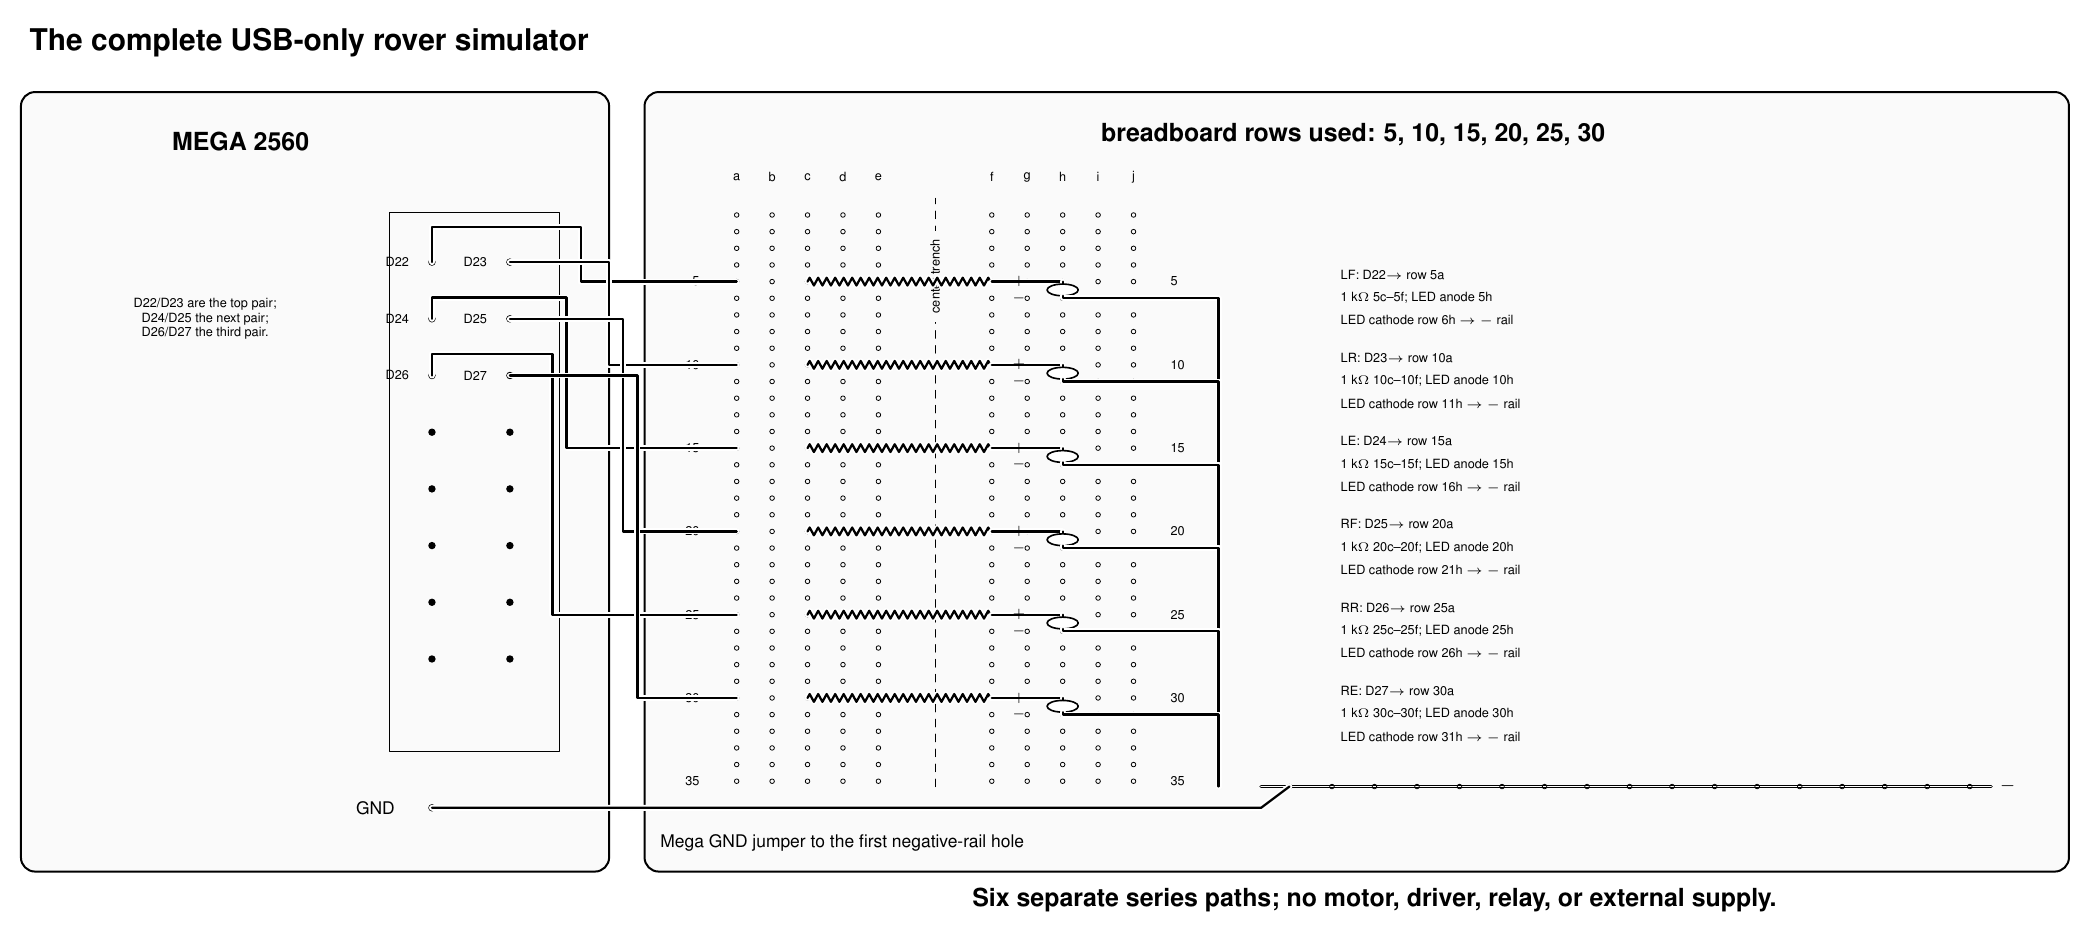
\includegraphics[width=\linewidth]{021-rover-layout.png}

\small\textit{The paired Mega header and breadboard coordinates are literal.
Every output has its own resistor and LED; only the cathode returns join at the
negative rail. The first hole of that rail returns to Mega GND.}
\end{center}

\begin{tabularx}{\linewidth}{@{}l X@{}}
\toprule
Signal & Complete path\\
\midrule
LF & D22 to 5a; 1 k\(\Omega\) from 5c to 5f; LED long leg at 5h,
short leg at 6h; 6j to negative rail\\
LR & D23 to 10a; resistor 10c--10f; long leg 10h, short leg 11h;
11j to negative rail\\
LE & D24 to 15a; resistor 15c--15f; long leg 15h, short leg 16h;
16j to negative rail\\
RF & D25 to 20a; resistor 20c--20f; long leg 20h, short leg 21h;
21j to negative rail\\
RR & D26 to 25a; resistor 25c--25f; long leg 25h, short leg 26h;
26j to negative rail\\
RE & D27 to 30a; resistor 30c--30f; long leg 30h, short leg 31h;
31j to negative rail\\
Return & first negative-rail hole to a labeled Mega GND pin\\
\bottomrule
\end{tabularx}

Unplug USB before moving a wire. The LED long leg is the anode. If the body
has a flat edge, that edge usually marks the short cathode leg; check the
actual LED before placing it.

\section{Build in three quick wins}

\textbf{Win 1---one imaginary wheel.} Build LF, LR, and LE on rows 5, 10, and
15. Upload the sketch. You should see left-side forward intent and later the
turn. If these three work, the left half of the story is already visible.

\textbf{Win 2---the rover appears.} Add RF, RR, and RE on rows 20, 25, and 30.
Both sides now drive forward together. During the turn the direction banks
disagree on purpose: that is how a two-wheel rover pivots.

\textbf{Win 3---the obstacle trick.} Watch near 2.5 seconds. Both enable lamps
go dark for a full second because the synthetic range drops from 500 mm to
150 mm. Nothing is pressed and no sensor is wired; the observation is a fixed,
replayable part of the sketch. At 3.5 seconds the clear range returns.

Each payoff depends on the earlier wiring. A missing resistor path, reversed
LED, shared row, or wrong Mega pin removes the matching character from the
story instead of creating a separate test chore.

\newpage
\section{Read the twelve-second story}

\begin{tabularx}{\linewidth}{@{}l X X@{}}
\toprule
Moment & What the six lamps show & What is happening\\
\midrule
startup & six dark; then D13 on & objects acquired before route intent\\
first act & LF, LE, RF, RE & both imaginary wheels forward\\
near 2.5 s & LE and RE dark & synthetic obstacle holds both sides stopped\\
after 3.5 s & route lamps resume & fresh clear range releases the hold\\
turn & opposite direction patterns, with a brief all-dark gap & requested
reversal waits for \texttt{MotorIntent} dead time\\
finish & all six dark & route ended with stopped intent\\
12 s & D13 and all six dark & fixed automatic shutdown released outputs\\
\bottomrule
\end{tabularx}

Small timing differences in LED brightness are normal because the enable
signals use duty values. The ordering is deterministic: identical timestamps
and observations produce identical controller snapshots.

\begin{lstlisting}[style=adkcpp]
void loop ()
{
    observeSimulatedRange  (nowUs);
    observeSimulatedWheels (now);
    decideRoverMotion      (now);
    actuateMotorEvidence   (now);
}
\end{lstlisting}

The canonical loop keeps the story in dependency order: observe, decide,
actuate. Serial is unnecessary; the six lamps are the primary result.

\section{Change the adventure}

\begin{enumerate}
  \item Change the near distance from 150 mm to 100 mm. Predict why the visible
        story stays the same: both values remain inside the stop threshold.
  \item Move the obstacle window from 2.5--3.5 seconds to 1.5--2.5 seconds.
        The blackout moves earlier without changing a wire.
  \item Change the first route step from eight edges to four. The turn should
        arrive earlier, proving the route data drives the story.
  \item Swap the physical LF and RF LEDs. Decide which facts remain true and
        which labels become misleading.
\end{enumerate}

\section{If a character disappears}

\begin{tabularx}{\linewidth}{@{}l X@{}}
\toprule
What you see & Inspect with USB unplugged\\
\midrule
Exactly one lamp never lights & its numbered Mega pin, resistor row, LED
polarity, and cathode jumper\\
Three left or three right lamps fail & the corresponding D22--D24 or D25--D27
header positions\\
Several unrelated lamps copy each other & accidental shared breadboard rows
or signal jumpers touching\\
Directions work but one enable stays dark & D24 or D27 and its complete series
path\\
No obstacle blackout & confirm the Lesson 021 sketch was uploaded, not Lesson
020\\
Any lamp remains after 12 seconds & reset once; if repeated, unplug USB\\
\bottomrule
\end{tabularx}

\section{What the repository checks behind the scenes}

Automated tests replay every route action, obstacle hysteresis boundaries,
stop dominance, stale or invalid range, wheel faults, route timeouts,
rollover, restart, shutdown, and byte-identical traces. Arduino compilation
and size checks cover the Mega sketch. Those checks protect the project
without becoming learner paperwork.

\section{Why there are no real wheels}

The software emits \emph{intent}; LEDs make that intent visible. Real motion
would require an exactly identified driver and motor, primary datasheets,
measured stall current, a separate current-limited load supply, flyback and
thermal design, a rated physical power disconnect, guarding, and physical
evidence. None is authorized by resemblance to a retail listing. This lesson
therefore ends at the safer and more useful USB-only simulator.

\vfill
\small
Status: host verified; no physical observation is claimed. The HTML lesson,
canonical sketch, and automated tests remain the current reference.
\end{document}
